\documentclass{article}
\usepackage[margin=1in]{geometry}
\usepackage{url}
\usepackage{forest}
\usepackage{tabu}
\usepackage{listings}
\usepackage{amsmath}
\usepackage{amsfonts}
\usepackage{float}
\usepackage{color}
\usepackage{multicol}
\usepackage[colorlinks = true,
            linkcolor = blue,
            urlcolor  = blue,
            citecolor = blue,
            anchorcolor = blue]{hyperref}
\usepackage{subfig}
\usepackage[font=small,labelfont=bf]{caption} % Required for specifying 
                                              % captions to tables and figures

\newcommand{\MYhref}[3][blue]{\href{#2}{\color{#1}{#3}}}%

\definecolor{dkgreen}{rgb}{0,0.6,0}
\definecolor{gray}{rgb}{0.5,0.5,0.5}
\definecolor{mauve}{rgb}{0.58,0,0.82}

\lstset{frame=tb,
  language=Java,
  aboveskip=3mm,
  belowskip=3mm,
  showstringspaces=false,
  columns=flexible,
  basicstyle={\small\ttfamily},
  numbers=none,
  numberstyle=\tiny\color{gray},
  keywordstyle=\color{blue},
  commentstyle=\color{dkgreen},
  stringstyle=\color{mauve},
  breaklines=true,
  breakatwhitespace=true,
  tabsize=3
}

\title{CPSC 524 Assignment 2: Area of the Mandelbrot Set}
\author{Rami Pellumbi\thanks{M.S., Statistics \& Data Science}}
\date{\today}

\begin{document}

\maketitle

\newpage 

\section{Introduction}

This assignment focuses on assessing the performance gains achievable through 
the application of loop directives and tasks in parallelizing the computation 
of the Mandelbrot set area. The basis for this study is a serial algorithm 
designed for this task, detailed as follows:

\begin{enumerate}
    \item We begin by defining a rectangular region in the complex plane, denoted as \textbf{R}. This region is bounded by the lower-left corner $-2.0 + 0.0i$ and the upper-right corner $0.5 + 1.25i$.
    \item This region \textbf{R} is then discretized into a grid of cells, each having a side length of 0.001 units. The set of all possible lower-left corner coordinates of these cells is represented by $T$, defined as:
    \begin{align*}
        T := \{(x, y) : x \in X, y \in Y \},
    \end{align*}
    where 
    \begin{align*}
        X &= \{x \in \mathbb{R} : x = -2.0 + n * 0.001, -2.0 \leq x < 0.5, n \in \mathbb{N}\}, \\
        Y &= \{y \in \mathbb{R} : y = 0.0 + n * 0.001, 0.0 \leq y < 1.25, n \in \mathbb{N}\}.
    \end{align*}
    A cell is uniquely defined by its lower-left corner coordinate $(x, y) \in X \times Y$. 
    We denote such a cell by $C_{x,y}$, and the set of all such cells is $C := \{C_{x, y}: (x, y) \in T\}$.
    
    A few clarifying remarks:
    \begin{itemize}
        \item The cardinality of $X$ is $$\lvert X \rvert = \frac{0.5 - (-2.0)}{0.001} = 2500.$$
        \item The cardinality of $Y$ is $$\lvert Y \rvert = \frac{1.25 - 0.0}{0.001} = 1250.$$
        \item The cardinality of $T$ is $$\lvert T \rvert = \lvert X \rvert \cdot \lvert Y \rvert = 2500 \cdot 1250 = 3125000.$$
    \end{itemize}
    
    \item For each cell $C_{x, y} \in C$, a random point $c$ within the cell is generated.
    \item The Mandelbrot update $z \leftarrow z^2 + c$ is iteratively computed for this random point $c$, for up to 25,000 iterations.
    \begin{enumerate}
        \item If the condition $\lvert z \rvert^2 > 4$ is met at any iteration, the point $c$ is marked as being outside the Mandelbrot set.
        \item Conversely, if all 25,000 iterations are completed without meeting this condition, the point $c$ is considered to be inside the Mandelbrot set.
    \end{enumerate}
    
    Let $N_I$ and $N_O$ denote the total number of points that are inside and outside the Mandelbrot set, respectively.
    \item The area estimate for the Mandelbrot set is computed as:
    \begin{align*}
        A = 2.0 \cdot \frac{N_I}{N_O + N_I} \cdot \text{Area}(\textbf{R}),
    \end{align*}
    where $\text{Area}(\textbf{R}) = 2.5 \times 1.25 = 3.125$.
\end{enumerate}

\section{Project Organization}

The project is laid out to provide a clean separation of source files, header files, compiled objects, and documentation. 

\begin{multicols}{2}
    \begin{forest}
        for tree={
            font=\ttfamily,
            grow'=0,
            child anchor=west,
            parent anchor=south,
            anchor=west,
            calign=first,
            edge path={
                \noexpand\path [draw, \forestoption{edge}]
                (!u.south west) +(7.5pt,0) |- node[fill,inner sep=1.25pt] {} (.child anchor)\forestoption{edge label};
            },
            before typesetting nodes={
                if n=1
                {insert before={[,phantom]}}
                {}
            },
            fit=band,
            before computing xy={l=15pt},
        }
    [a2
        [bin/]
        [docs/]
        [include/]
        [out/]
        [src/]
        [build-run-part1.sh]
        [build-run-part2.sh]
        [build-run-part3.sh]
        [build-run-part4.sh]
        [data.Rmd]
        [Makefile]
    ]
    \end{forest}
    \columnbreak
    \begin{itemize}
        \item \textbf{bin/}: The \texttt{bin} folder holds compiled objects and executable files, centralizing the output of the compilation process.
        \item \textbf{docs/}: This folder contains LaTeX files and other documentation materials that pertain to the report.
        \item \textbf{include/}: Here, all the header files (\texttt{.h}) are stored. These headers contain function prototypes and static inline functions used across different benchmarks.
        \item \textbf{out/}: The \texttt{out} folder stores the outputs from each task. Each subdirectory is of the relevant task. It also houses the csv files generated by the programs.
        \item \textbf{src/}: This directory houses the source files (\texttt{.c}) that make up the benchmarks.
        \item \textbf{Shell Scripts}: The shell scripts are at the root directory and are used to submit the job for the relevant task to slurm via \texttt{sbatch}. 
        \item \textbf{data.Rmd}: This R Markdown file is used to generate the tables and plots from the output csv files for the report.
        \item \textbf{Makefile}: This Makefile has undergone extensive modifications to support the project hierarchy. It is engineered to handle the appropriate linking of shared libraries and integration of common code components, ensuring a seamless compilation process.
    \end{itemize}
\end{multicols}

\section{Code Explanation, Compilation, and Execution}

This section outlines the steps required to build and execute the code. The provided Bash scripts automate the entire process, 
making it straightforward to compile and run the code. All the below steps assume 
you are in the root of the project directory.

\subsection{Automated Building and Execution}
\begin{itemize}
    \item \textbf{Part 1: Serial Program} 
    There are two implementation of the serial program (to be elaborated in Section 4). 
    The command \texttt{sbatch build-run-part1.sh} will compile and run the files:
    \begin{itemize}
        \item \texttt{mandseq.c}: standard, slightly optimized, serial implementation of the algorithm.
        \item \texttt{mandseq-avx.c} more advanced implementation with AVX 512 instructions.
    \end{itemize}
    The output of the experiments will be in \texttt{out/serial.csv}.
    
    \item \textbf{Part 2: OMP Loop Directives}
    There are multiple programs run in Part 2. The programs associated with part 2 are:
    \begin{itemize}
        \item \texttt{mandomp.c}: extending \texttt{mandseq.c} to use OMP loop directives.
        \item \texttt{mandomp-avx.c}: extending \texttt{manseq-avx.c} to use OMP loop directives.
        \item \texttt{mandomp-ts.c}: a copy of \texttt{mandomp.c} using \texttt{drand-ts.c} for thread safe random number generation (RNG).
        \item \texttt{mandomp-ts-avx.c} a copy of \texttt{mandomp-avx.c} using \texttt{drand-ts.c} for thread safe RNG.
        \item \texttt{mandomp-collapse.c} a modification of \texttt{mandomp-ts.c} to support the collapse clause.
        \item \texttt{mandomp-collapse-avx.} a modification of \texttt{mandomp-ts-avx.c} to support the collapse clause.
    \end{itemize}
    The script \texttt{build-run-part2.sh} validates the weird behavior of the non thread safe RNG, shows how the fix 
    in \texttt{drand-ts.c} fixes the issue, and assesses the thread safe code against multiple thread counts and multiple 
    schedules. To run all the experiments, execute \texttt{sbatch build-run-part2.sh}. The results are stored in 
    \texttt{out/omp.csv}.

    \item \textbf{Part 3: OMP Tasks}
    In part 3, only the AVX version of the program is adopted to OMP Tasks. There are multiple programs run in Part 3. The programs associated with part 3 are:
    \begin{itemize}
        \item \texttt{mandomp-tasks.c}: extending \texttt{mandseq-avx.c} to use OMP tasks. One thread creates tasks and one task is created per batch of cells. 
        \item \texttt{mandomp-tasks-columns.c}: extending \texttt{mandomp-tasks.c} to instead create one task per column. One thread creates tasks.
        \item \texttt{mandomp-ts-columns-shared.c}: a copy of \texttt{mandomp-tasks-columns.c} but now all threads create tasks.
    \end{itemize}
    The script \texttt{build-run-part3.sh} assesses the area and wall clock time of the above progrmas. 
    To run all the experiments, execute \texttt{sbatch build-run-part3.sh}. The results are stored in \texttt{out/tasks.csv}.

    \item \textbf{Part 4: Parallel RNG}
    In part 4, \texttt{mandomp-ts-avx.c} is modified into \texttt{mandomp-ts-avx-parallel.c}. It makes use of the parallel random 
    number generator in \texttt{drand-ts.c}.
    To run all the experiments, execute \texttt{sbatch build-run-part4.sh}. The results are stored in \texttt{out/omp-parallel.csv}. 
\end{itemize}

\subsection{Post-Build Objects and Executables}
Upon successful compilation and linking, an \texttt{obj/} directory will be generated within the root directory. 
This directory will contain the compiled output files. Additionally, the executable files for running each part will be 
situated in the \texttt{bin/} directory.

\subsection{Output Files From \texttt{sbatch}}
The output files generated from running the code by submitting the relevant Bash script via \texttt{sbatch} will be 
stored in the relevant subdirectory of the \texttt{out} directory. 

\section{Serial Implementation}
The serial implementation was first written in the standard way to achieve a runtime of approximately 
49.2 seconds. After some searching, an optimized implementation using AVX 256 instructions was found.\footnote{Source: \MYhref{https://polarnick.com/blogs/other/cpu/gpu/sse/opencl/openmp/2016/10/01/mandelbrot-set-sse-opencl.html}{https://polarnick.com/blogs/other/cpu/gpu/sse/opencl/openmp/2016/10/01/mandelbrot-set-sse-opencl.html}} 
This source was rewritten to the assignment at hand using AVX 512 instructions found in the \MYhref{https://www.intel.com/content/www/us/en/docs/intrinsics-guide/index.html}{intel intrinsics guide}. 
The serial runtime was improved to approximately 17.7 seconds using AVX 512 instructions. 
The serial implementation and all subsequent implementations make use of the provided 
random number generator seeded at value 12345.

\subsection{Standard Implementation}
\subsubsection{Implementation}
First, we iterate over the cells in \textbf{R} by a double for loop 
through the sets $X$ and $Y$. Concretely, the below loops iterate over all $(x, y) \in T$.
For each cell $C_{x, y}$, we generate a random coordinate inside the cell and perform the 
mandelbrot iteration on it. Since we are performing $N = 3125000$ iterations total, we 
can simply count the number of cells inside the mandelbrot set and then compute $N_O = N - N_I$. 
This gets rid of any conditional checks in the loop helping optimize.
The resulting for loop is:
\begin{lstlisting}
    int N = 3125000, N_I = 0;
    for (size_t n = 0; n < 2500; n++)
    {
        double current_bottom_left_x = -2.0 + CELL_SIDE_LENGTH * n;
        double max_x = current_bottom_left_x + CELL_SIDE_LENGTH;
        for (size_t m = 0; m < 1250; m++)
        {
            double current_bottom_left_y = 0.0 + CELL_SIDE_LENGTH * m;
            double max_y = current_bottom_left_y + CELL_SIDE_LENGTH;
            // Get a random x and y inside of the cell
            double random_x = current_bottom_left_x + (max_x - current_bottom_left_x) * drand();
            double random_y = current_bottom_left_y + (max_y - current_bottom_left_y) * drand();
            // mandelbrot_iteration returns 0 if outside the set, else 1
            N_I +=  mandelbrot_iteration(random_x, random_y);
        }
    }
    int N_O = N - N_I; 
\end{lstlisting}
The \texttt{mandelbrot\_iteration} function checks if the complex number with real part 
\texttt{random\_x} and imaginary part \texttt{random\_y}. The implementation is 
found in \texttt{mandelbrot.h}. The function is static inlined to allow for portability 
between the multiple programs and is elaborated below:
\begin{lstlisting}
   static inline int mandelbrot_iteration(double c_re, double c_im, size_t max_iterations)
   {
       double z_re = 0.0, z_im = 0.0; // start at 0
       double magnitude_squared = 0.0;
   
       for (size_t i = 0; i < max_iterations; i++)
       {
           // compute the real part of z in the update
           double temp_re = z_re * z_re - z_im * z_im + c_re; 
           // compute the imaginary part of z in the update
           z_im = (z_re + z_re) * z_im + c_im; 
           z_re = temp_re;
           magnitude_squared = z_re * z_re + z_im * z_im;
           // break if we diverged
           if (magnitude_squared > 4.0) { return 0; }
       }
       return 1;
   } 
\end{lstlisting}
The update rule was done more optimally than just doing $z^2 + c$ via the pseudocode 
found in \MYhref{https://en.wikipedia.org/wiki/Mandelbrot_set}{Wikipedia}.
It is worth noting that complex numbers were manually handled via tracking two real numbers 
rather than using the \texttt{double complex} type from the \texttt{<complex.h>}. Using the complex 
library resulted in atrociously bad performance relative to using just doubles. This seems to 
be a \MYhref{https://stackoverflow.com/questions/42659668/stdcomplex-multiplication-is-extremely-slow}{a common issue}.

\subsubsection{Results}
Running the standard implementation 3 times, the following results were obtained:
\begin{table}[H]
    \centering
    \caption{Serial Wall Clock Time and Area - Standard Algorithm}
    \fontsize{12}{14}\selectfont
    \begin{tabular}[t]{r|r|l|r|r}
    \hline
    num\_threads & seed & program & wc\_time & area\\
    \hline
    1 & 12345 & serial & 49.25816 & 1.506648\\
    \hline
    1 & 12345 & serial & 49.25670 & 1.506648\\
    \hline
    1 & 12345 & serial & 49.25700 & 1.506648\\
    \hline
    \end{tabular}
\end{table}
\noindent The wall clock time is roughly 49.2 seconds. 
Each execution yielded a stable area estimate of 1.506648, 
which is a minor deviation from the 1.506632 value cited in the assignment guidelines. 
In our algorithm, we adopted a column-wise selection strategy for iterating through the cells \( C_{x,y} \). 
Specifically, we looped over all available \( y \) values for a given fixed \( x \). 
The state of the random number generator evolves as we traverse the cells, 
occupying distinct positions in its sequence. 
This results in different sampling points within each cell for each traversal scheme and thus 
will result in different points being selected in each $C_{x,y}$, potentially yielding a 
different area estimate. 

\subsection{AVX 512 Implementation}
The Intel\textsuperscript{\textregistered} Xeon\textsuperscript{\textregistered} 
Platinum 8268 processor supports AVX-512, which allows for simultaneous operations 
on eight double-precision floating-point numbers. The AVX-512 version of this 
algorithm is implemented using the Intel AVX-512 instruction set, as detailed 
in Intel's Intrinsics Guide\footnote{Source: \MYhref{https://www.intel.com/content/www/us/en/docs/intrinsics-guide/index.html}{Intel Intrinsics Guide}}. 
This capability enables the concurrent sampling of points for eight \( C_{x,y} \) 
values and checks whether they belong to the Mandelbrot set.

\subsubsection{Implementation}
We still iterate over the cells in \textbf{R} by a double loop through the sets 
$X$ and $Y$, but now we process 8 $y$ values at a time. Since 1250 is not a multiple of 8, the remaining 
values are processed in a cleanup loop that is the standard serial implementation:
\begin{lstlisting}
    for (size_t n = 0; n < 2500; n++)
    {
        double current_bottom_left_x = -2.0 + CELL_SIDE_LENGTH * n;
        double max_x = current_bottom_left_x + CELL_SIDE_LENGTH;

        // compute 8 y-values simultaneously
        for (size_t m = 0; m < 1250 / 8 * 8; m += 8)
        {
            // need to generate the 16 random numbers for the 8 cells
            for (int i = 0; i < 8; ++i)
            {
                random_x[i] = drand(); // pre-allocated arrays for 8 doubles
                random_y[i] = drand();
            }
            // load the random numbers into a 512 bit register via an unaligned load
            __m512d random_numbers_x = _mm512_loadu_pd(random_x);
            __m512d random_numbers_y = _mm512_loadu_pd(random_y);

            // get the 8 bottom left and top left y values for this iteration of the loop
            __m512d bottom_left_y_values = _mm512_add_pd(
                _mm512_set1_pd(0.0),
                _mm512_add_pd(_mm512_set1_pd(m * CELL_SIDE_LENGTH), pxs_deltas512));
            __m512d top_left_y_values = _mm512_add_pd(
                _mm512_set1_pd(CELL_SIDE_LENGTH),
                bottom_left_y_values);

            // compute the random coordinates for the 8 cells
            __m512d x_values = _mm512_fmadd_pd(
                random_numbers_x,
                _mm512_set1_pd(max_x - current_bottom_left_x),
                _mm512_set1_pd(current_bottom_left_x));
            __m512d y_values = _mm512_fmadd_pd(
                random_numbers_y,
                _mm512_sub_pd(top_left_y_values, bottom_left_y_values),
                bottom_left_y_values);

            // Assess the 8 c values concurrently
            __mmask8 diverged_indices = mandelbrot_iteration_avx(
                x_values,
                y_values,
                MAX_ITERATIONS);

            // the 1's in this mask are the iterations that did NOT diverge
            __mmask8 indices_in_set = ~diverged_indices;
            int count = _popcnt32((unsigned int)indices_in_set);
            number_of_cells_inside_mandelbrot_set += count;

            total_iterations += 8;
        }

        // cleanup by performing the standard serial implementation
        for (size_t m = 1250 / 8 * 8; m < 1250; m++)
        {
            // standard serial implementation
        }
    }
\end{lstlisting}
\noindent The \texttt{mandelbrot\_iteration\_avx} assesses the 8 sampled points from the 8 $C_{x,y}$ values simultaneously as follows:
\begin{lstlisting}
    static inline __mmask8 mandelbrot_iteration_avx(__m512d x_values,
                                                         __m512d y_values,
                                                         size_t max_iterations)
    {
        // These are the 8 z values
        __m512d z_re = _mm512_set1_pd(0.0);
        __m512d z_im = _mm512_set1_pd(0.0);

        // 8 bit mask. 1 means that the c value at that index has diverged.
        __mmask8 diverged_indices = 0;

        // Assess the 8 c values concurrently
        for (size_t iteration = 0; iteration < max_iterations; iteration++)
        {
            // componentwise: z_re = z_re * z_re + z_im * z_im + c_re
            __m512d xsn = _mm512_add_pd(_mm512_sub_pd(
                                            _mm512_mul_pd(z_re, z_re),
                                            _mm512_mul_pd(z_im, z_im)),
                                        x_values);

            // componentwise: z_im = 2 * z_re * z_im + c_im
            __m512d ysn = _mm512_add_pd(_mm512_mul_pd(
                                            _mm512_add_pd(
                                                z_re,
                                                z_re),
                                            z_im),
                                        y_values);

            // Update only those positions where diverged_indices is zero
            __m512d new_z_re = _mm512_mask_mov_pd(z_re, ~diverged_indices, xsn);
            __m512d new_z_im = _mm512_mask_mov_pd(z_im, ~diverged_indices, ysn);
            z_re = new_z_re;
            z_im = new_z_im;

            // compute the magnitude squared componentwise
            __m512d magnitude_squared = _mm512_add_pd(
                _mm512_mul_pd(z_re, z_re),
                _mm512_mul_pd(z_im, z_im));

            // Generate a mask for numbers that have diverged (magnitude squared > 4)
            __mmask8 maskDiverged = _mm512_cmp_pd_mask(magnitude_squared,
                                                    _mm512_set1_pd(4.0),
                                                    _CMP_GT_OS);

            // Update diverged_indices using bitwise OR operation
            diverged_indices |= maskDiverged;

            // Break if all indices have diverged
            if (diverged_indices == 0xFF)
            {
                return diverged_indices;
            }
        }

        return diverged_indices;
    }
\end{lstlisting}
\noindent A shortcoming of this algorithm is that it requires all indices to diverge 
in order to break. So there is a worst case scenario where 7 cells near immediately 
diverge but one cell completes all the iterations. A more advanced implementation might 
find a way around this issue.

\subsubsection{Results}
Running the AVX 512 implementation 3 times, the following results were obtained:
\begin{table}[H]
    \centering
    \caption{Serial Wall Clock Time and Area - AVX Algorithm}
    \fontsize{12}{14}\selectfont
    \begin{tabular}[t]{r|r|l|r|r}
    \hline
    num\_threads & seed & program & wc\_time & area\\
    \hline
    1 & 12345 & serial-avx & 17.75959 & 1.506656\\
    \hline
    1 & 12345 & serial-avx & 17.75925 & 1.506656\\
    \hline
    1 & 12345 & serial-avx & 17.75885 & 1.506656\\
    \hline
    \end{tabular}
\end{table}
\noindent The wall clock time for the algorithm leveraging AVX-512 was measured 
at approximately 17.8 seconds. This represents a speedup of approximately 2.76 times 
compared to the standard implementation.\footnote{
    This performance gain is suboptimal compared to the theoretical 8 times speedup. Several factors contribute to this disparity. 
    Memory bandwidth limitations can cause delays in loading data into SIMD registers, 
    reducing the effective speedup. The inherent latencies and throughputs of AVX-512 instructions, 
    as well as the overheads associated with loading and storing data from and to SIMD registers, can also affect performance. 
    Moreover, non-vectorizable portions of the code can further dilute the anticipated gains.
} Each 
run of the algorithm produced an area estimate of 1.506656. 
This value differs from both the standard serial implementation's estimate 
and the value suggested by the assignment guide. While the same random numbers as the standard implementation 
were used in each iteration—ensured by synchronizing the state of the random number generator—the 
hypothesis for the discrepancy in the area estimate is that AVX-512 intrinsics 
operate with a distinct floating-point precision profile. This different precision 
profile could alter the computational outcome, leading to the observed variation in the area estimate.

\section{OpenMP Loop Directives}
Next, the serial implementation was modified to use loop directives to create parallel, 
multithreaded versions of the serial implementation. To handle this, the double 
for loop is wrapped in the \texttt{omp parallel} directive; explicitly instructing 
the compiler to parallelize the chosen block of code. The first for loop is then tagged 
with the \texttt{omp for} directive; instructing the compiler to distribute loop 
iterations within the team of threads that encounters this work-sharing construct. The environment variables 
\texttt{OMP\_NUM\_THREADS} and \texttt{OMP\_SCHEDULE} are used to control the core count (one thread per core) 
and scheduling, respectively.

\subsection{Parallel threads using \texttt{omp for} - No Scheduling}
Each thread has private variables \texttt{total\_iterations\_th} and \texttt{number\_of\_cells\_in\_mandelbrot\_set\_th} 
which tally the total iterations that thread performed and the number of points in the mandelbrot set that thread determined, respectively. Additionally, 
each thread instantiates its own seed.
At the end, each threads private variables are added atomically to the shared variables:
\begin{itemize}
    \item \texttt{number\_of\_cells\_inside\_mandelbrot\_set},
    \item \texttt{total\_iterations}.
\end{itemize}
For the AVX version, each thread also needs two 8 length double arrays for the random numbers. Explicitly, the AVX algorithm is something like:\footnote{The non AVX version is 
near identical. The only difference is each thread does not require an array to store the random numbers in since they can be computed on the fly and are not loaded into a register.}
\begin{lstlisting}
    #pragma omp parallel shared(number_of_cells_inside_mandelbrot_set, total_iterations) private(number_of_cells_inside_mandelbrot_set_th, total_iterations_th, random_x, random_y) default(none)
    {
        dsrand(seed); // each thread initializes a seed
        random_x = (double *)malloc(8 * sizeof(double));
        random_y = (double *)malloc(8 * sizeof(double));
        number_of_cells_inside_mandelbrot_set_th = 0;
        total_iterations_th = 0;

        #pragma omp for
        for (size_t m = 0; m < 2500; ++m)
        {
            // AVX code from prior
            for (size_t n = 0; n < 1250 / 8 * 8; n += 8) { ... }
            // standard code from prior
            for (size_t n = 1250 / 8 * 8; n < 1250 ; ++n) { ... }
        }
        // add each threads results to the desired totals
        #pragma omp atomic
        number_of_cells_inside_mandelbrot_set += number_of_cells_inside_mandelbrot_set_th;

        #pragma omp atomic
        total_iterations += total_iterations_th;

        free(random_x);
        free(random_y);
    }
\end{lstlisting}
The \texttt{omp atomic} directive ensures the addition of each threads results to the shared variables is done atomically.\footnote{
    In particular, it ensures that race conditions are avoided through direct control of concurrent threads that might read or write to or from the particular memory location. 
    It allows for more efficient concurrent algorithms due to the use of fewer locks than \texttt{omp critical}. 
    \MYhref{https://www.ibm.com/docs/sk/xl-c-aix/13.1.0?topic=processing-pragma-omp-atomic}{https://www.ibm.com/docs/sk/xl-c-aix/13.1.0?topic=processing-pragma-omp-atomic}
}

\subsubsection{Lack of Thread Safety}
The above algorithm is run using the base \texttt{drand} implementation with the environment variables:
\begin{itemize}
   \item \texttt{OMP\_NUM\_THREADS} set to 2.
   \item \texttt{OMP\_SCHEDULE} not set.
\end{itemize}
This runs the algorithm with two cores (one thread per core) and no scheduling. The results are:
\begin{table}[H]
    \centering
    \caption{OMP Wall Clock Time and Area - drand}
    \centering
    \fontsize{12}{14}\selectfont
    \begin{tabular}[t]{r|r|l|r|r}
    \hline
    num\_threads & seed & program & wc\_time & area\\
    \hline
    2 & 12345 & standard & 42.09501 & 1.506796\\
    \hline
    2 & 12345 & standard & 42.09643 & 1.506670\\
    \hline
    2 & 12345 & standard & 42.08855 & 1.506686\\
    \hline
    2 & 12345 & avx & 15.16014 & 1.506838\\
    \hline
    2 & 12345 & avx & 15.17255 & 1.506796\\
    \hline
    2 & 12345 & avx & 15.16531 & 1.506812\\
    \hline
    \end{tabular}
\end{table}
\noindent Table 3 shows both a performance improvement over the serial implementation and 
the algorithm computing a different area estimate each run. The performance improvement for 
both the standard and AVX serial algorithm using two threads is approximately 1.2$\times$ faster.

\subsubsection{Thread Safe Random Number Generation}
The differing area estimates are due to the lack of thread safe random number generation. In particular, 
multiple threads may be modifying the same seed value causing unstable random number 
generation. This is fixed by modifying the static seed variable in \texttt{drand.c} to be \texttt{threadprivate}. 
In particular, the \texttt{omp threadprivate} directive makes the static block-scope variable private to each 
thread. This prevents multiple threads from updating the same seed value and ensures each thread 
computes its own random numbers. The implementation is a one line change to \texttt{drand.c} and is done in \texttt{drand-ts.c} 
to make running the experiments easier. Explicitly:
\begin{lstlisting}
    static uint64_t seed_ts;
    
    // ensures each thread is modifying it's own seed
    #pragma omp threadprivate(seed_ts)
    
    void dsrand_ts(unsigned s)
    {
        seed_ts = s - 1;
        printf("Seed_ts = %lu. RAND_MAX = %d.\n", seed_ts, RAND_MAX);
    }
    
    double drand_ts(void)
    {
        seed_ts = 6364136223846793005ULL * seed_ts + 1;
        return ((double)(seed_ts >> 33) / (double)RAND_MAX);
    } 
\end{lstlisting}
A problem with this fix in particular is each thread will use the same sequence of random numbers. 
This is remedied in section 7. Using \texttt{dsrand\_ts} and \texttt{drand\_ts} instead of \texttt{dsrand} and \texttt{drand} in the 
2 thread no schedule experiment yields:
\begin{table}[H]
    \centering
    \caption{OMP Wall Clock Time and Area - drand-ts}
    \centering
    \fontsize{12}{14}\selectfont
    \begin{tabular}[t]{r|r|l|r|r}
    \hline
    num\_threads & seed & program & wc\_time & area\\
    \hline
    2 & 12345 & omp-ts & 41.87915 & 1.506622\\
    \hline
    2 & 12345 & omp-ts & 41.86007 & 1.506622\\
    \hline
    2 & 12345 & omp-ts & 41.85505 & 1.506622\\
    \hline
    2 & 12345 & omp-avx-ts & 15.01974 & 1.506716\\
    \hline
    2 & 12345 & omp-avx-ts & 15.02008 & 1.506716\\
    \hline
    2 & 12345 & omp-avx-ts & 15.01922 & 1.506716\\
    \hline
    \end{tabular}
\end{table}
\noindent We observe the same wall clock performance, but this fix now allows for reproducible area values for a fixed number of threads. 
Moving forward, we run all experiments with the thread safe random number generator.

\subsubsection{Loop Directives Wall Clock Time and Area Across Thread Counts - Using \texttt{drand-ts}}
The algorithm is now run with \texttt{OMP\_NUM\_THREADS} set to 1, 2, 4, 12, and 24 cores (one thread per core) with no scheduling. 
The results are: 
\begin{table}[H]
    \centering
    \caption{OMP Wall Clock Time and Area Across Threads - No Scheduling}
    \centering
    \fontsize{12}{14}\selectfont
    \begin{tabular}[t]{l|r|r|r}
    \hline
    program & num\_threads & wc\_time & area\\
    \hline
    omp-avx-ts & 1 & 17.631131 & 1.506656\\
    \hline
    omp-avx-ts & 2 & 15.021128 & 1.506716\\
    \hline
    omp-avx-ts & 4 & 8.000733 & 1.506778\\
    \hline
    omp-avx-ts & 12 & 3.447970 & 1.506652\\
    \hline
    omp-avx-ts & 24 & 1.937948 & 1.506664\\
    \hline
    serial & 1 & 49.25670 & 1.506648 \\
    \hline 
    omp-ts & 1 & 49.006569 & 1.506648\\
    \hline
    omp-ts & 2 & 41.859844 & 1.506622\\
    \hline
    omp-ts & 4 & 22.352743 & 1.506532\\
    \hline
    omp-ts & 12 & 9.674459 & 1.506682\\
    \hline
    omp-ts & 24 & 5.409102 & 1.506800\\
    \hline
    \end{tabular}
\end{table}
\noindent We observe that increasing the thread count results in faster execution of both the 
standard and AVX implementation. The performance improvement factor is the same across both algorithms. 
The serial version has the same area estimate as the parallel version with one thread, which makes sense as it 
is precisely the same algorithm. As the number of thread counts increases, our random number generator is 
instantiated on more threads. The algorithm is also processing a different batch of cells for each thread and thus 
the area estimate is bound to change as a different point is chosen in each cell for varying thread counts.

\subsection{Parallel threads using \texttt{omp for} - With Scheduling}
We add the \texttt{schedule(runtime)} clause to the \texttt{for} directive to allow 
for setting the scheduling of iterations to threads. 
Now, for each thread count \texttt{OMP\_NUM\_THREADS} set to 2, 4, 12, and 24 cores, we assess \texttt{OMP\_SCHEDULE} set to: 
\texttt{schedule(static, 1)}, \texttt{schedule(static, 100)}, \texttt{schedule(dynamic)}, \texttt{schedule(dynamic, 250)}, and \texttt{schedule(guided)}. Respectively, 
these options perform:
\begin{itemize}

\item \textbf{schedule(static, 1)}:
  \begin{itemize}
    \item Method: Each thread receives one iteration at a time until all iterations are exhausted. Iterations are allocated in a round-robin fashion.
    \item Pros \& Cons: Minimal overhead but poor load balance if iterations have varying computational costs.
  \end{itemize}

\item \textbf{schedule(static, 100)}:
  \begin{itemize}
    \item Method: Iterations are divided into chunks of 100 and statically assigned to threads.
    \item Pros \& Cons: Low overhead and since the number of iterations is divisible by 100 there are no threads left idle.
  \end{itemize}

\item \textbf{schedule(dynamic)}:
  \begin{itemize}
    \item Method: Iterations are dynamically assigned to threads as they become available.
    \item Pros \& Cons: High overhead but excellent load balancing.
  \end{itemize}

\item \textbf{schedule(dynamic, 250)}:
  \begin{itemize}
    \item Method: Each thread dynamically grabs chunks of 250 iterations from the loop.
    \item Pros \& Cons: Once the 2500 iterations to schedule have been assigned we expect no performance gain above about 10 threads.
  \end{itemize}

\item \textbf{schedule(guided)}:
  \begin{itemize}
    \item Method: Dynamic assignment of decreasingly sized blocks of iterations to each thread.
    \item Pros \& Cons: Aims to balance overhead and load by initially assigning large chunks and reducing the size dynamically.
  \end{itemize}
\end{itemize}
The average wall clock time and area for the AVX algorithm for each thread and schedule were:
\begin{table}[H]
    \centering
    \caption{OMP Wall Clock Time and Area Across Threads - All Schedules AVX}
    \centering
    \fontsize{12}{14}\selectfont
    \begin{tabular}[t]{l|l|r|r|r}
    \hline
    program & schedule & num\_threads & wc\_time & area\\
    \hline
    omp-avx-ts & dynamic & 2 & 8.857233 & 1.506857\\
    \hline
    omp-avx-ts & dynamic & 4 & 4.426543 & 1.506663\\
    \hline
    omp-avx-ts & dynamic & 12 & 1.478229 & 1.506761\\
    \hline
    omp-avx-ts & dynamic & 24 & 0.741666 & 1.506795\\
    \hline
    omp-avx-ts & dynamic,250 & 2 & 9.398375 & 1.506794\\
    \hline
    omp-avx-ts & dynamic,250 & 4 & 5.694130 & 1.506746\\
    \hline
    omp-avx-ts & dynamic,250 & 12 & 4.477652 & 1.506758\\
    \hline
    omp-avx-ts & dynamic,250 & 24 & 4.479328 & 1.506758\\
    \hline
    omp-avx-ts & guided & 2 & 8.857341 & 1.506644\\
    \hline
    omp-avx-ts & guided & 4 & 4.500216 & 1.506787\\
    \hline
    omp-avx-ts & guided & 12 & 1.484397 & 1.506694\\
    \hline
    omp-avx-ts & guided & 24 & 0.745663 & 1.506713\\
    \hline
    omp-avx-ts & static,1 & 2 & 8.851426 & 1.506732\\
    \hline
    omp-avx-ts & static,1 & 4 & 4.429402 & 1.506760\\
    \hline
    omp-avx-ts & static,1 & 12 & 1.482386 & 1.506800\\
    \hline
    omp-avx-ts & static,1 & 24 & 0.743956 & 1.506802\\
    \hline
    omp-avx-ts & static,100 & 2 & 8.854995 & 1.506648\\
    \hline
    omp-avx-ts & static,100 & 4 & 5.102193 & 1.506622\\
    \hline
    omp-avx-ts & static,100 & 12 & 2.041134 & 1.506880\\
    \hline
    omp-avx-ts & static,100 & 24 & 1.939225 & 1.506736\\
    \hline
    \end{tabular}
\end{table}
\noindent The area estimate differs amongst different schedules for the same thread count. This 
indicates that the cells are being traversed in a different order for the different schedules 
and thus a different point is likely sampled within each cell (which on the boundary matters 
a lot for determining if we are inside or outside the set). For the wall clock time, we notice:
\begin{itemize}
    \item \texttt{dynamic}: There is a consistent decrease in wall clock time as
    the number of threads increases. We are lead to believe that the load is 
    being well-distributed for a chunk size of 1 and that all threads are working efficiently.
    \item \texttt{dynamic, 250} The wall clock time decreases until 12 threads 
    and then plateaus. A too-large chunk size is leading to less efficient use of 
    threads as thread count increases. Indeed, we expect 10 threads to grab the 
    2500 iterations to schedule over and the remaining threads above 10 are left completely idle. This 
    is precisely what is observed.
    \item \texttt{guided}: Very similar in performance to \texttt{dynamic}. This 
    makes sense since the chunk size decreases over time and the threads seem 
    to work more efficiently in this manner.
    \item \texttt{static,1}: This has the same time decrease pattern as \texttt{dynamic}. 
    The chunk size being set to 1 appears to allow for a good work distribution despite the 
    potential overhead.
    \item \texttt{static, 100}: The time decrease here is less smooth than that of 
    \texttt{static, 1}. This indicates some threads are either being left idle or 
    inefficiently used. There is little performance gain between 12 and 24 threads.
\end{itemize}
It is worth noting that wall clock time is significantly impacted by even one slow thread. 
Since the density of cells inside the Mandelbrot set is non constant as we iterate through the columns, 
threads that have to handle the center are bound to take more time. Thus, the 
\texttt{dynamic, guided,} and \texttt{static,1} options handle work distribution better than 
when we assign threads a large chunk of work as the threads in charge of the center will undoubtedly take more time.
The next table shows the results for the standard algorithm, where the exact same conclusion is drawn.
\begin{table}[H]
    \centering
    \caption{OMP Wall Clock Time and Area Across Threads - All Schedules Standard}
    \centering
    \fontsize{12}{14}\selectfont
    \begin{tabular}[t]{l|l|r|r|r}
    \hline
    program & schedule & num\_threads & wc\_time & area\\
    \hline
    omp-ts & dynamic & 2 & 24.546266 & 1.506733\\
    \hline
    omp-ts & dynamic & 4 & 12.279111 & 1.506719\\
    \hline
    omp-ts & dynamic & 12 & 4.093797 & 1.506722\\
    \hline
    omp-ts & dynamic & 24 & 2.049885 & 1.506824\\
    \hline
    omp-ts & dynamic,250 & 2 & 25.915077 & 1.506752\\
    \hline
    omp-ts & dynamic,250 & 4 & 15.846655 & 1.506792\\
    \hline
    omp-ts & dynamic,250 & 12 & 12.539101 & 1.506682\\
    \hline
    omp-ts & dynamic,250 & 24 & 12.539795 & 1.506682\\
    \hline
    omp-ts & guided & 2 & 24.598179 & 1.506790\\
    \hline
    omp-ts & guided & 4 & 12.471653 & 1.506759\\
    \hline
    omp-ts & guided & 12 & 4.132643 & 1.506768\\
    \hline
    omp-ts & guided & 24 & 2.055091 & 1.506711\\
    \hline
    omp-ts & static,1 & 2 & 24.550046 & 1.506662\\
    \hline
    omp-ts & static,1 & 4 & 12.277485 & 1.506794\\
    \hline
    omp-ts & static,1 & 12 & 4.103413 & 1.506824\\
    \hline
    omp-ts & static,1 & 24 & 2.055128 & 1.506882\\
    \hline
    omp-ts & static,100 & 2 & 24.671857 & 1.506674\\
    \hline
    omp-ts & static,100 & 4 & 14.196153 & 1.506664\\
    \hline
    omp-ts & static,100 & 12 & 5.696408 & 1.506728\\
    \hline
    omp-ts & static,100 & 24 & 5.445335 & 1.506714\\
    \hline
    \end{tabular}
\end{table}
\noindent We conclude that certain types of scheduling improve the load balance amongst 
threads for loop directives for both the standard and AVX algorithm. 

\subsection{Parallel threads using \texttt{omp for} - With Collapsing \& Scheduling}
Next, the loop uses the collapse clause; increasing the number of loop chunks that
the runtime system can schedule across the threads.. The source code was slightly 
modified to allow for collapsing. In particular, no code can be inbetween the two loops 
iterating through $X$ and $Y$ and thus the code for computing the $X$ values is moved to the 
inner most loop. In the AVX algorithm, since there is a cleanup loop, we have to collapse twice - once for the AVX code and once for the standard cleanup.
The AVX algorithm adjustments are shown to emphasize the changes:
\newpage
\begin{lstlisting}
    #pragma omp parallel // insert same shared, private
    { // insert same setup
        #pragma omp for collapse(2) schedule(runtime)
        for (size_t n = 0; n < NUM_X_ITERATIONS; n++)
        {
            for (size_t m = 0; m < NUM_Y_PS; m += 8)
            {
                // to support collapse have to compute the current bottom left x for all  y values now
                // insert same AVX sequential code
            }
        }

        // to support collapsing the cleanup iterations must be their own collapse
        #pragma omp for collapse(2) schedule(runtime)
        for (size_t i = 0; i < NUM_X_ITERATIONS; ++i)
        {
            for (size_t j = NUM_Y_PS; j < NUM_Y_ITERATIONS; ++j)
            {
                // have to compute x for all y values to support collapsing
                // insert same standard sequential code
            }
        } // insert same cleanup
    }
\end{lstlisting}
The results were measured for \texttt{OMP\_NUM\_THREADS} set to 2, 4, 12, and 24 cores and \texttt{OMP\_SCHEDULE} set to
the same options as prior.
The next table shows the results from collapsing across scheduling options for the AVX algorithm
\begin{table}[H]
    \centering
    \caption{OMP Wall Clock Time and Area Across Threads - All Schedules With Collapse AVX}
    \centering
    \fontsize{12}{14}\selectfont
    \begin{tabular}[t]{l|l|r|r|r}
    \hline
    program & schedule & num\_threads & wc\_time & area\\
    \hline
    omp-collapse-avx & dynamic & 2 & 8.924948 & 1.506725\\
    \hline
    omp-collapse-avx & dynamic & 4 & 4.463100 & 1.506759\\
    \hline
    omp-collapse-avx & dynamic & 12 & 1.489609 & 1.506655\\
    \hline
    omp-collapse-avx & dynamic & 24 & 0.748752 & 1.506757\\
    \hline
    omp-collapse-avx & dynamic,250 & 2 & 8.917002 & 1.506840\\
    \hline
    omp-collapse-avx & dynamic,250 & 4 & 4.459263 & 1.506713\\
    \hline
    omp-collapse-avx & dynamic,250 & 12 & 1.487800 & 1.506748\\
    \hline
    omp-collapse-avx & dynamic,250 & 24 & 0.747705 & 1.506653\\
    \hline
    omp-collapse-avx & guided & 2 & 8.948330 & 1.506829\\
    \hline
    omp-collapse-avx & guided & 4 & 4.544421 & 1.506701\\
    \hline
    omp-collapse-avx & guided & 12 & 1.504375 & 1.506810\\
    \hline
    omp-collapse-avx & guided & 24 & 0.751079 & 1.506727\\
    \hline
    omp-collapse-avx & static,1 & 2 & 8.982337 & 1.506750\\
    \hline
    omp-collapse-avx & static,1 & 4 & 4.554585 & 1.506808\\
    \hline
    omp-collapse-avx & static,1 & 12 & 1.599819 & 1.506694\\
    \hline
    omp-collapse-avx & static,1 & 24 & 0.803146 & 1.506684\\
    \hline
    omp-collapse-avx & static,100 & 2 & 8.925599 & 1.506888\\
    \hline
    omp-collapse-avx & static,100 & 4 & 4.460062 & 1.506850\\
    \hline
    omp-collapse-avx & static,100 & 12 & 1.494543 & 1.506714\\
    \hline
    omp-collapse-avx & static,100 & 24 & 0.750147 & 1.506734\\
    \hline
    \end{tabular}
\end{table}
\noindent The collapse clause offers no noticeably enhanced improvements to \texttt{static, 1}, \texttt{dynamic}, and \texttt{guided}. 
However, it significantly improves the prior ill performing \texttt{dynamic, 250} and \texttt{static, 100}.
This makes sense for the source code. In the non-collapsed code, there are 2500 
iterations to schedule over and the \texttt{dynamic, 250} cannot make use of more than 10 threads. 
However, in the collapsed code, there are 2500*1250 iterations to schedule over in the standard 
algorithm (2500 * 158 in the AVX version) and thus each thread can be kept busy. 
In a similar fashion, the load is better distributed for chunk sizes of 100 across the 2500*1250 schedulable 
iterations for \texttt{static, 100}, which no longer has any one thread handle an entire chunk of the center.

The performance being the same for the other scheduling options is likely because the non-collapse code, 
which has 2500 iterations to schedule over, gives a sufficient number of 
schedulable chunks to achieve good load balance. In the collapsed version, there 
are more chunks to schedule and it appears the overhead of scheduling these chunks 
outweighs any performance gain. Additionally, we no longer make use of caching the x values for each stride of y. 
Below is the table of values for the standard algorithm, where the exact same conclusions are drawn.
\begin{table}[H]
    \centering
    \caption{OMP Wall Clock Time and Area Across Threads - All Schedules With Collapse Standard}
    \centering
    \fontsize{12}{14}\selectfont
    \begin{tabular}[t]{l|l|r|r|r}
    \hline
    program & schedule & num\_threads & wc\_time & area\\
    \hline
    omp-collapse & dynamic & 2 & 24.793561 & 1.506799\\
    \hline
    omp-collapse & dynamic & 4 & 12.412081 & 1.506779\\
    \hline
    omp-collapse & dynamic & 12 & 4.180311 & 1.506715\\
    \hline
    omp-collapse & dynamic & 24 & 2.123831 & 1.506677\\
    \hline
    omp-collapse & dynamic,250 & 2 & 24.672736 & 1.506713\\
    \hline
    omp-collapse & dynamic,250 & 4 & 12.336788 & 1.506789\\
    \hline
    omp-collapse & dynamic,250 & 12 & 4.111878 & 1.506702\\
    \hline
    omp-collapse & dynamic,250 & 24 & 2.058562 & 1.506671\\
    \hline
    omp-collapse & guided & 2 & 24.747149 & 1.506708\\
    \hline
    omp-collapse & guided & 4 & 12.602658 & 1.506728\\
    \hline
    omp-collapse & guided & 12 & 4.168920 & 1.506780\\
    \hline
    omp-collapse & guided & 24 & 2.067399 & 1.506884\\
    \hline
    omp-collapse & static,1 & 2 & 24.743476 & 1.506694\\
    \hline
    omp-collapse & static,1 & 4 & 12.381558 & 1.506850\\
    \hline
    omp-collapse & static,1 & 12 & 4.130896 & 1.506624\\
    \hline
    omp-collapse & static,1 & 24 & 2.068478 & 1.506822\\
    \hline
    omp-collapse & static,100 & 2 & 24.667321 & 1.506718\\
    \hline
    omp-collapse & static,100 & 4 & 12.334259 & 1.506728\\
    \hline
    omp-collapse & static,100 & 12 & 4.119450 & 1.506808\\
    \hline
    omp-collapse & static,100 & 24 & 2.063424 & 1.506754\\
    \hline
    \end{tabular}
\end{table}

\subsection{Comparing It All}
Looking at tables of value can make it difficult to compare results. We assess 
the performance of collapsing vs. not collapsing across thread counts across schedules 
graphically to observe the lack of performance gains that scheduling and collapsing provide 
the algorithm in the following figure:
\begin{figure}[H]
    \centering
    \subfloat[\centering Standard Algorithm Performance For Each Schedule Across Thread Counts]{{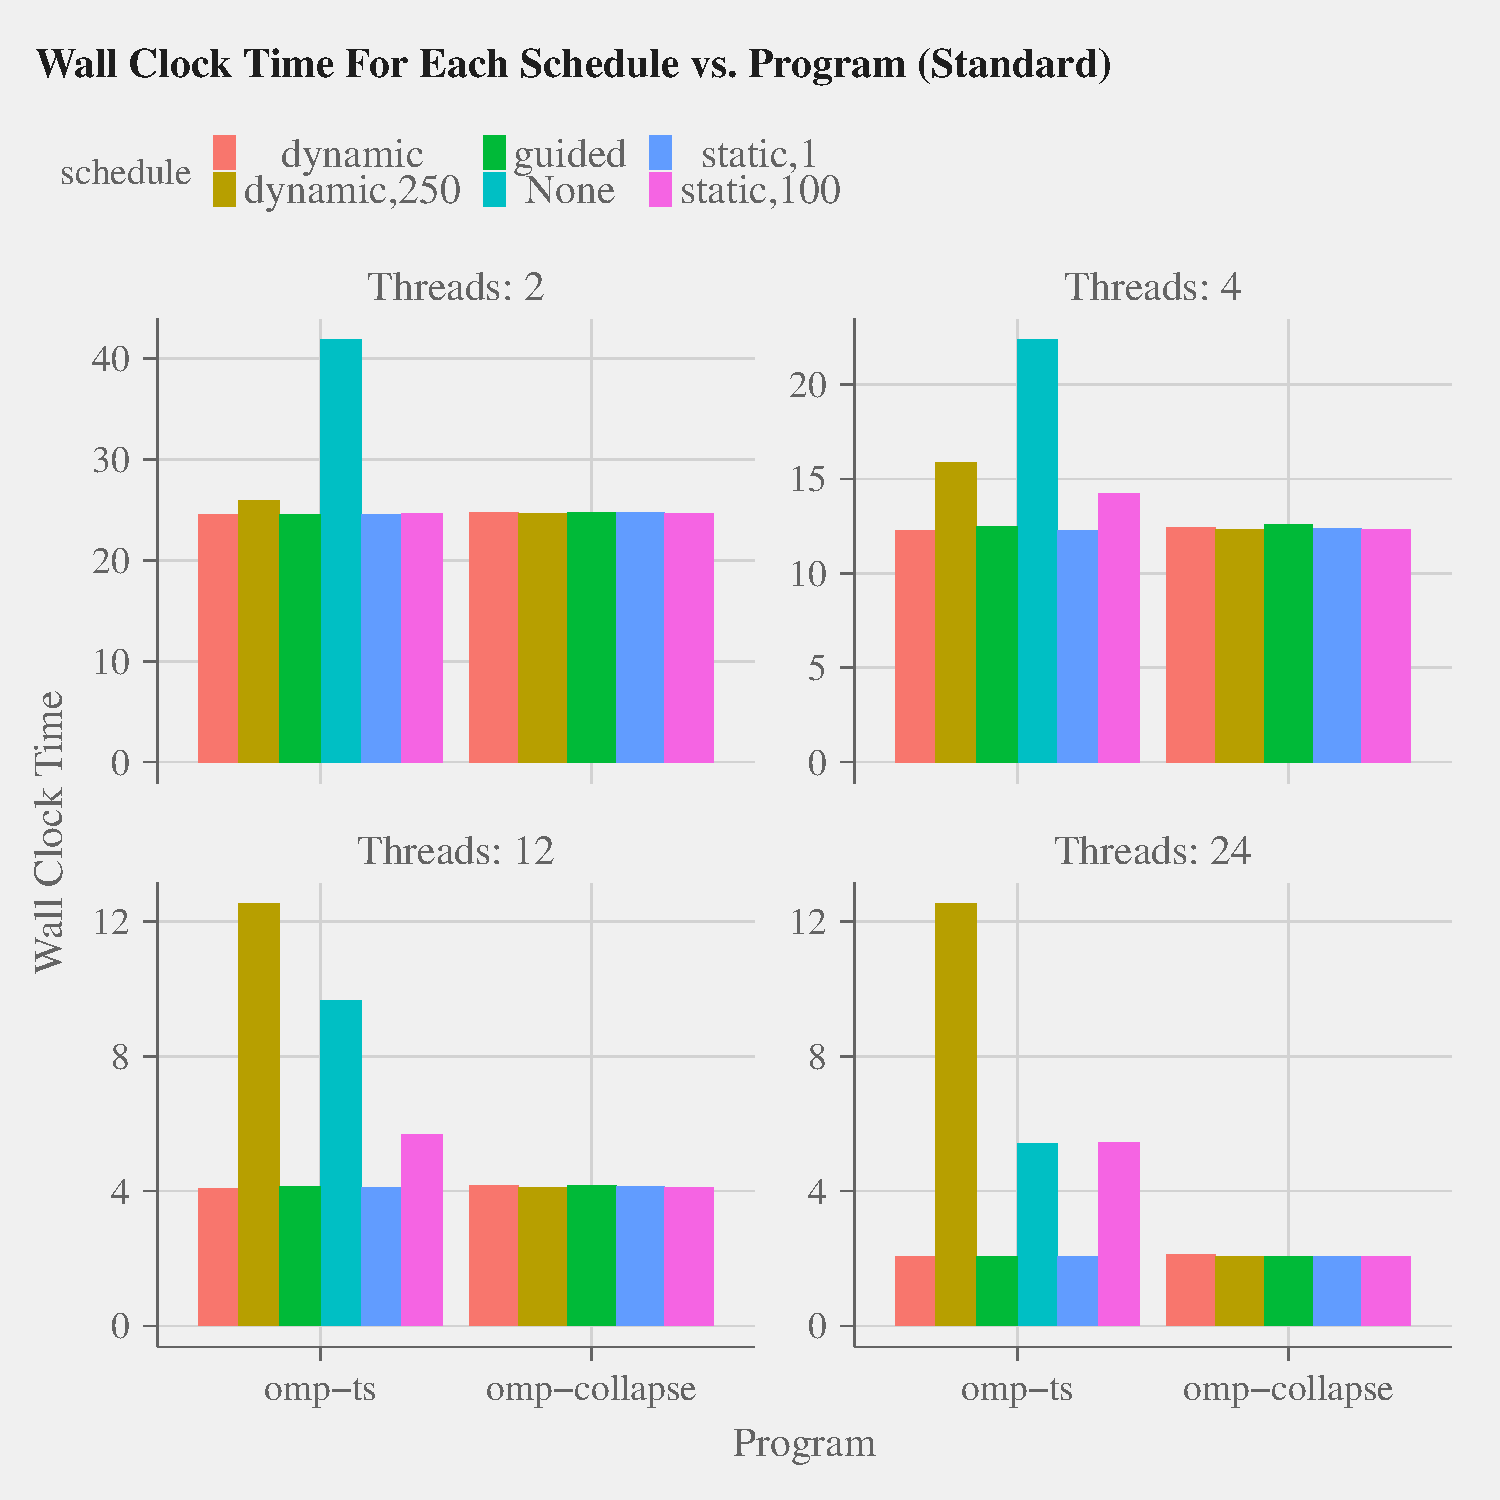
\includegraphics[width=0.48\linewidth]{q2-img.pdf} }}
    \subfloat[\centering AVX Algorithm Performance For Each Schedule Across Thread Counts]{{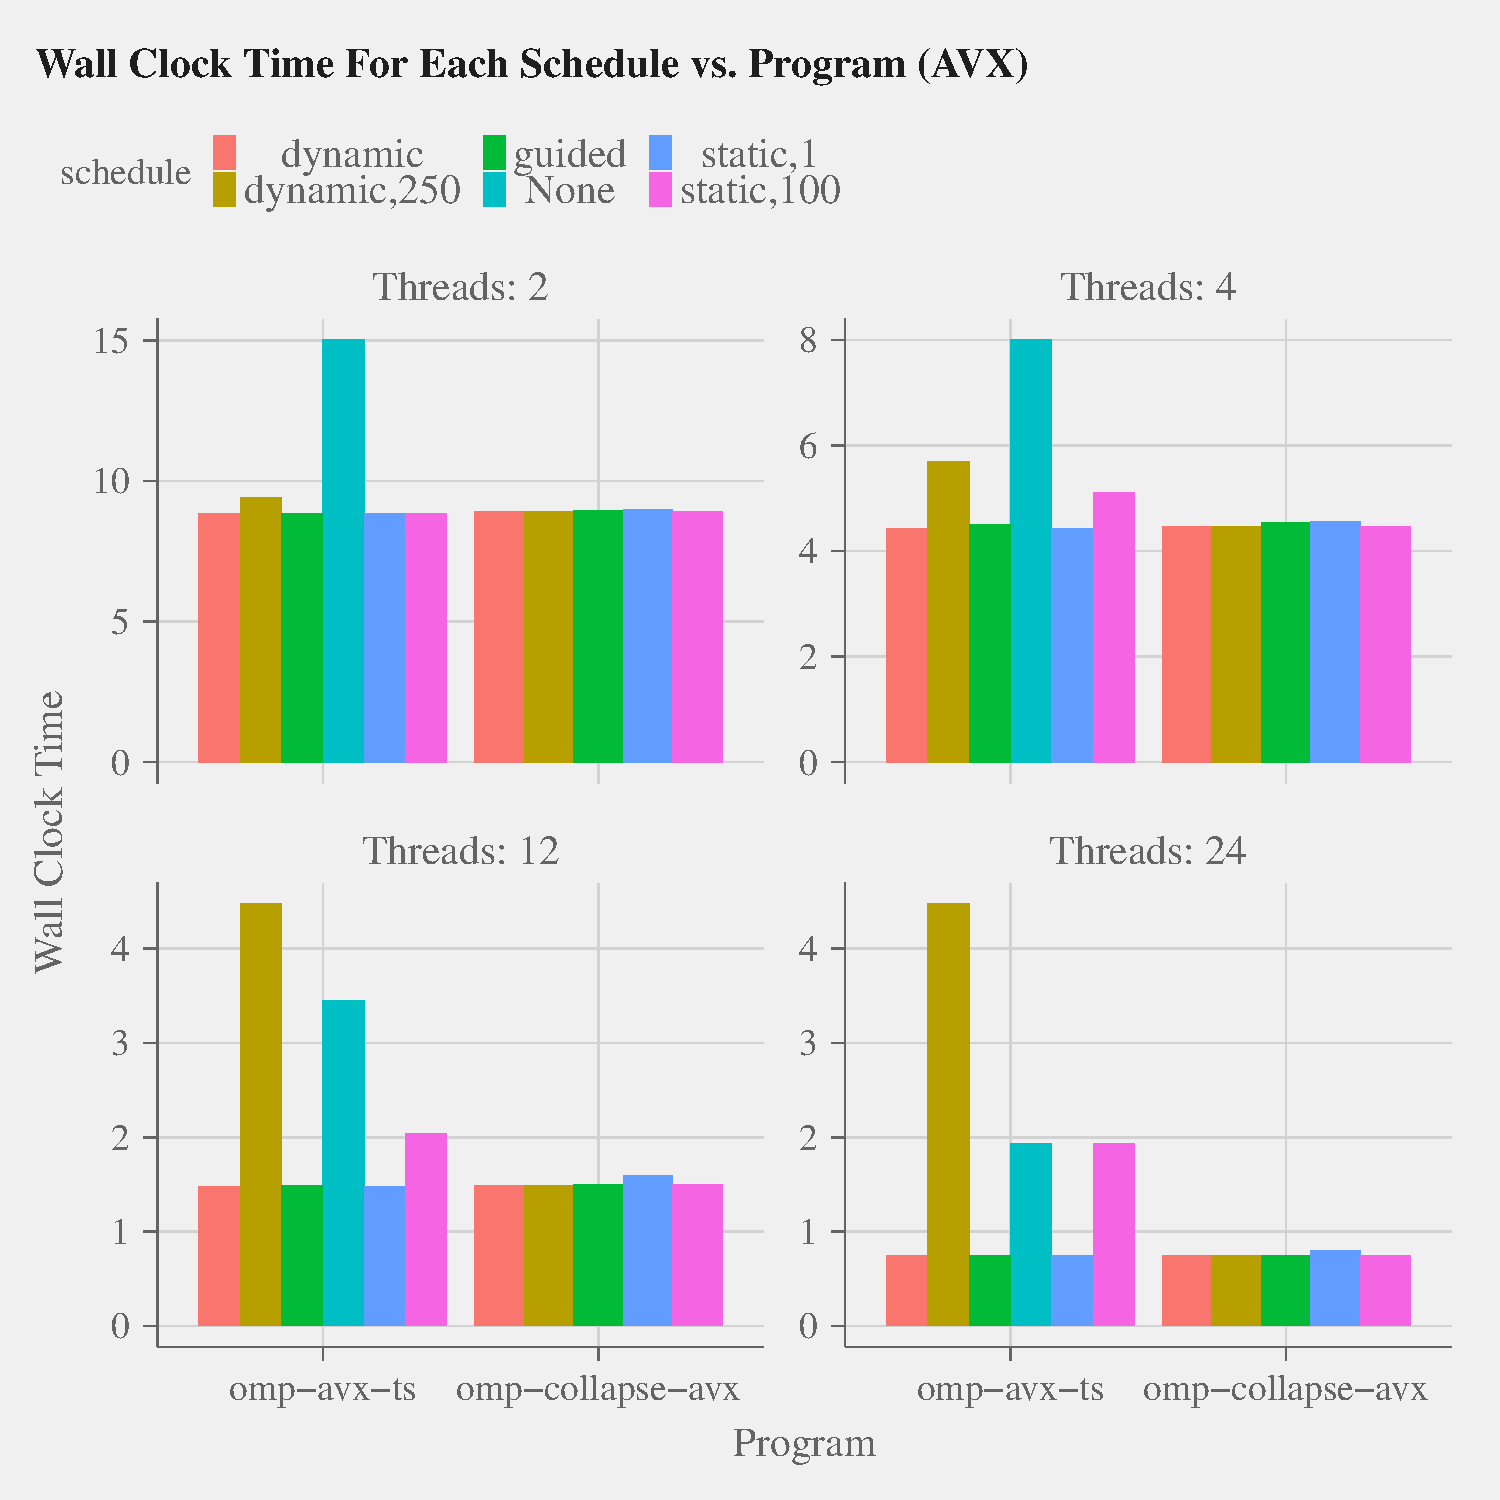
\includegraphics[width=0.48\linewidth]{q2-img-avx.pdf} }}
\end{figure}
\noindent It is visibly observable that the wall clock change between collapsing and non collapsing 
is similar for the schedules \texttt{static, 1}, \texttt{dyamic}, and \texttt{guided} while the 
wall clock time for \texttt{static, 100} and \texttt{dynamic, 250} is signicantly improved as 
thread count increases for the collapsed program.

\section{OpenMP Tasks}
The next task takes the serial implementation and uses OpenMP tasks to parallelize it. Only 
the AVX version is operated on in this step to compare to the loop directives performance. First, 
a program is created in which each cell or batch of cells constitutes a task and one thread 
is dedicated to creating all the tasks. Then, a program is created that treats each 
column of cells as a task and one thread is dedicated to creating all the tasks. Finally, 
the program is modified to so that each column of cells is treated as a task but all threads are able to create tasks.

\subsection{One Task Per Cell Batch}
Since the AVX algorithm operates on 8 cells at once, 
each batch of 8 cells is its own task. The cleanup loop, which operates on one cell at once, has each individual cell 
created as a task. To implement this, we:
\begin{itemize}
    \item Take the \texttt{mandseq-avx.c} and wrap the double for loop in the parallel directive - with almost same sharing and private rules as \texttt{mandomp-avx.c}.
    \item Wrap the double for loop in the omp single directive - specifying that the for loop must run a single thread. 
    \item Wrap the \texttt{mandelbrot\_iteration\_avx} and \texttt{mandelbrot\_iteration} functions in the omp task directive.
    \item Each task updates the global counters \texttt{total\_iterations} and \texttt{number\_of\_cells\_inside\_mandelbrot\_set} atomically instead of each thread having its own counter.
\end{itemize}
In total, $2500 * (1248 / 8 + (1250 - 1248)) = 395000$ tasks are created.
The average area and average time across core counts 1, 2, 4, 12, and 24 was:
\begin{table}[H]
    \centering
    \caption{OMP Tasks Clock Time and Area - Task Per Cell Batch}
    \fontsize{12}{14}\selectfont
    \begin{tabular}[t]{l|r|r|r}
    \hline
    program & num\_threads & wc\_time & area\\
    \hline
    per-cell-task & 1 & 17.771752 & 1.506656\\
    \hline
    per-cell-task & 2 & 8.950503 & 1.506656\\
    \hline
    per-cell-task & 4 & 4.534696 & 1.506656\\
    \hline
    per-cell-task & 12 & 1.657044 & 1.506656\\
    \hline
    per-cell-task & 24 & 0.963572 & 1.506656\\
    \hline
    \end{tabular}
    \end{table}
\noindent It is remarkable that for core count larger than 1 the task algorithm is twice as fast as any scheduled loop directive (same performance for 1 core). 
There is a possibility that the runtime system has more flexibility in scheduling tasks than in scheduling loop chunks, allowing it to do a better job of balancing the load. 
Another possibility for the speedup is now we are parallelizing just the the mandelbrot iteration function, which may have a faster longest thread runtime than the entire 
loop directive version.
The average area computation is consistent across all thread counts and equal to that of the sequential algorithm - which was not the case with any of the 
loop directive AVX algorithms. This is because tasks are being processed with the exact same random number sequence as in the sequential version.

\subsection{One Task Per Column - Single Thread Task Generation}
The program is modified so that for each $x$ value, one task is created (2500 tasks total). This is a simple change 
and the inner for loops on $y$ are wrapped in the task directive. The average area and average time across core counts 1, 2, 4, 12, and 24 was:
\begin{table}[H]
    \centering
    \caption{OMP Tasks Clock Time and Area - Task Per Column}
    \fontsize{12}{14}\selectfont
    \begin{tabular}[t]{l|r|r|r}
    \hline
    program & num\_threads & wc\_time & area\\
    \hline
    per-column-task & 1 & 17.584878 & 1.506656\\
    \hline
    per-column-task & 2 & 8.812490 & 1.506645\\
    \hline
    per-column-task & 4 & 4.432580 & 1.506692\\
    \hline
    per-column-task & 12 & 1.510451 & 1.506747\\
    \hline
    per-column-task & 24 & 0.777615 & 1.506649\\
    \hline
    \end{tabular}
\end{table}
\noindent For 2, 4, and 12 cores there is a minor performance gain. For 24 cores, the per column 
task is about 1.2x faster than the per cell task. It is still near double the speed of 
the omp for loop directives version. It is interesting to note that the area estimate now 
differs again as the core count varies. The reasoning is the random number generator 
is not on the same state for all $C_{x,y}$ and thus different points are assessed for 
inclusion.

\subsection{One Task Per Column - Multiple Threads Generating Tasks}
The program is modified so that all threads generate tasks. This is done by 
keeping the omp task directive as is, removing the omp single directive wrapping the for loops, 
and placing an omp parallel directive on the outermost for loop. Placing the omp for directive is necessary 
so that task creation is split evenly amongst the threads. Without it, every thread tries to create the 2500 tasks 
leading to a lot of errors. The average area and average time across core counts 1, 2, 4, 12, and 24 was:
\begin{table}[H]
    \centering
    \caption{OMP Tasks Clock Time and Area - Task Per Column Multithreaded Task Creation}
    \fontsize{12}{14}\selectfont
    \begin{tabular}[t]{l|r|r|r}
    \hline
    program & num\_threads & wc\_time & area\\
    \hline
    per-column-task-shared & 1 & 17.655240 & 1.506656\\
    \hline
    per-column-task-shared & 2 & 8.841601 & 1.506771\\
    \hline
    per-column-task-shared & 4 & 4.422934 & 1.506579\\
    \hline
    per-column-task-shared & 12 & 1.486727 & 1.506735\\
    \hline
    per-column-task-shared & 24 & 0.751839 & 1.506671\\
    \hline
    \end{tabular}
\end{table}
\noindent For 2, 4, 12, and 24 cores there is a minor performance gain over the prior program. 
We are still at near 2x speedup compared to the loop directive version. It appears the program is 
capable of load balancing the task creation and execution well even when threads are also busy creating tasks. The area 
estimates differ from when a single thread was creating all tasks. This is again due to the random number generator 
not being in the same state for all $C_{x,y}$ and thus different points are assessed for 
inclusion.

\section{Parallel Random Number Generation}
A shortcoming of the random number generator used throughout this project is that multiple threads 
may wind up using the same sequence of random numbers. This is due to the fact that each thread initiates itself 
at the same seed starting point and thus each thread could wind up using the exact same sequence of random numbers. 
One simple way to remedy this is via to give each thread its own starting point as a function of the seed. In this way, 
results are reproducible for the same seed but each thread will wind up using a different sequence of random numbers. 
Using Ian Foster's documented Leapfrog Method for creating a distributed number generator,
\footnote{Source: \MYhref{https://www.mcs.anl.gov/\~itf/dbpp/text/node116.html}{https://www.mcs.anl.gov/~itf/dbpp/text/node116.html}}
we implement the Leapfrog Method:
\begin{enumerate}
    \item Each thread needs to be initialized with a seed that is a function of the master seed and the thread's ID.
    \item The thread updates its seed by advancing the seed by the number of threads. E.g.,
    \begin{itemize}
        \item Thread 0 uses numbers at position 0, \texttt{NUM\_THREADS}, 2*\texttt{NUM\_THREADS},...
        \item Thread 1 uses numbers at position 1, \texttt{NUM\_THREADS} + 1, 2*\texttt{NUM\_THREADS} + 1,...
        \item Thread $i$ uses numbers at position $i$, \texttt{NUM\_THREADS} + $i$, 2*\texttt{NUM\_THREADS} + $i$,...
    \end{itemize}
\end{enumerate}
The following changes are made to \texttt{drand-ts.c}:
\newpage
\begin{lstlisting}
    static uint64_t seed_ts;
    // ensures each thread is modifying it's own seed
    #pragma omp threadprivate(seed_ts)
    
    // Advance the RNG state by `n` steps
    void leapfrog(uint64_t *seed, uint64_t n)
    {
        for (uint64_t i = 0; i < n; ++i)
        {
            *seed = 6364136223846793005ULL * (*seed) + 1;
        }
    }
    
    void dsrand_parallel_ts(unsigned s)
    {
        int thread_id = omp_get_thread_num();
    
        uint64_t master_seed = s - 1;
        seed_ts = master_seed;
    
        // Each thread leapfrogs `thread_id` steps from master_seed
        leapfrog(&seed_ts, thread_id);
    }
    
    double drand_parallel_ts()
    {
        // leapfrog the seed ahead num_threads
        int num_threads = omp_get_num_threads();
        leapfrog(&seed_ts, num_threads);
    
        return ((double)(seed_ts >> 33) / (double)RAND_MAX);
    }
\end{lstlisting}
The program \texttt{mandomp-ts-avx.c} is copied into \texttt{mandomp-ts-avx-parallel.c} and each thread 
invokes the function \texttt{dsrand\_parallel\_ts} to set its seed to the appropriate starting value. The function 
\texttt{drand\_parallel\_ts} gets the next random number for the thread by leaprogging the seed for that thread 
by the number of threads. The program is rerun with 24 cores with the best performing result from part 2. 
Since the results in part 2 were all so close, the absolute minimum wall clock time was chosen. 
This was when there was 24 cores and the schedule was \texttt{dynamic}. The average area and wall clock time are:
\begin{table}[H]
    \centering
    \caption{Investigating OMP Loop Directives with Parallel RNG}
    \fontsize{12}{14}\selectfont
    \begin{tabular}[t]{l|l|r|r|r}
    \hline
    program & schedule & num\_threads & wc\_time & area\\
    \hline
    omp-avx-ts & dynamic & 24 & 0.741666 & 1.506795\\
    \hline
    omp-avx-parallel-rng & dynamic & 24 & 0.753090 & 1.506693\\
    \hline
    \end{tabular}
\end{table}
\noindent The parallel rng does make a difference on the area estimate. I would 
have more confidence using the leapfrog method throughout to ensure the randomness 
in each thread is independent than that of other threads. Since the leapfrog method allows 
for reproducible results, there is no reason not to use a more parallel safe random number generator.
\end{document}

